\chapter{Introduction to Programming}

% Separate 'part' from 'section'.
\newpage

% This section discusses basic C language syntax.
\section{Basic Syntax}

% A \newpage should be placed at the end of every chapter.
\newpage


% This section runs through a detailed explanation of the classic 'Hello World' program.
%
% Line by line, the traditional "Hello World" tutorial program is deconstructed and explained in a
% detailed manner.
% 
% This section can be datched and compiled alone with a standalone TeX compiler.
\section{Program Structure}

\subsection{Core Tenants}
   \paragraph{}
      A program in C more or less consists of the same building blocks\smartcite{TUTPNT:1}:
      \begin{itemize}
         \item Preprocessor directives, like \verb;#include;;
         \item Functions, like \verb;main;;
         \item Variables;
         \item Statements and expressions;
         \item and comments.
      \end{itemize}

   \paragraph{}
      Let us take a look at one of the most widely used examples---

\subsection{Hello World}
   \paragraph{}
      In this part of the document, we're going to be touching on one of the foundational elements in teaching the C programming language: the `Hello World'
      program. Simply put, we are going to write a program that prints the line ``Hello, world!'' into the terminal where we can see it. For the sake of
      simplicity, each figure in this document will be done in Visual Studio Code, but I will, from time to time, include examples from other editors to
      show what may need to be done differently to achieve the same or similar result.

   \paragraph{}
      In order to accomplish this, we must first open our text editor and our command line interface (terminal) if they aren't already open. With those
      programs up and running, we must create the file that our code will reside in. (see Figure 2.1)

   \begin{figure}[h!]
      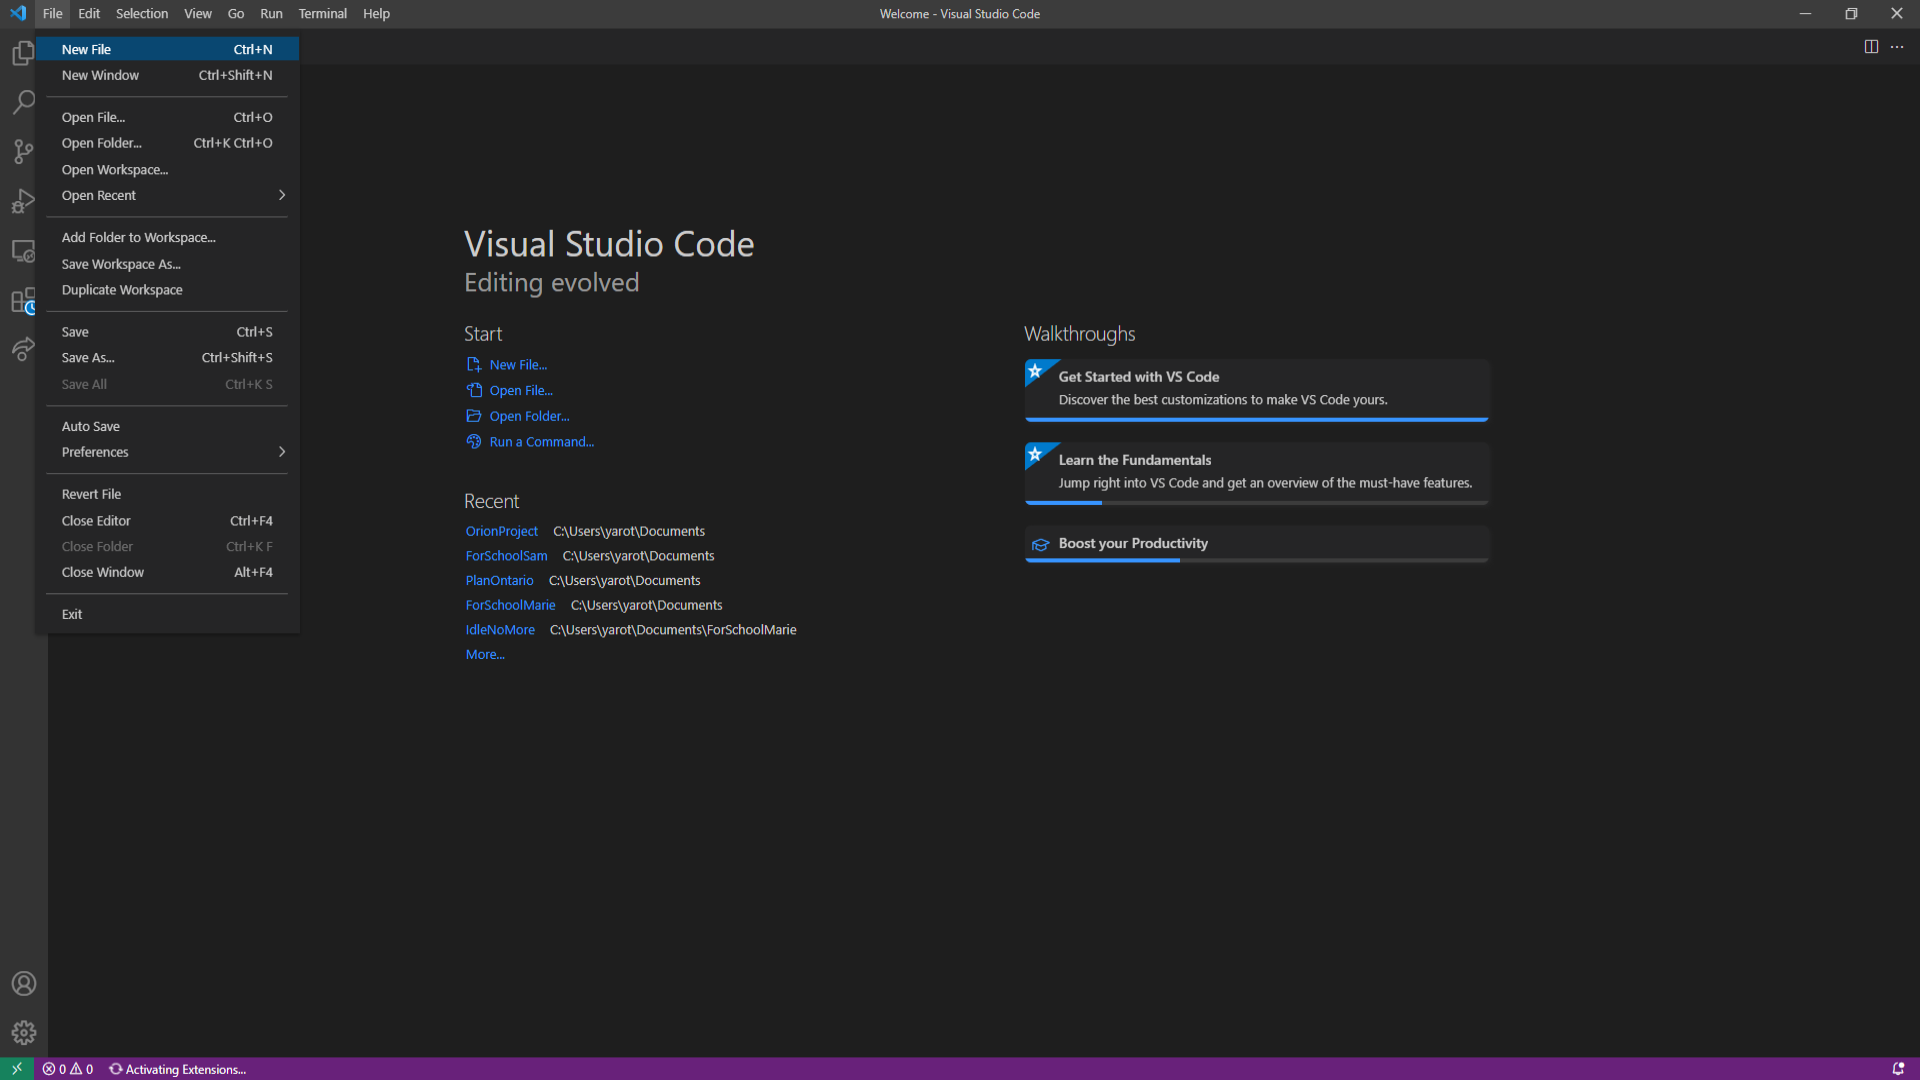
\includegraphics[width=\linewidth]{Figure1_VSCODE.png}
      \caption{Create the file by clicking on the ``New File'' button.}
      \label{fig:vscode_newfile}
   \end{figure}

   \paragraph{}
      Once the new file is created, we can begin by writing a few lines of code. Don't worry if the figure below is confusing as we will explain each
      individual line as we continue.

% A \newpage is necessary here to avoid splitting the figure in half.
\newpage

\begin{lstlisting}
// https://github.com/mnimi/intro_to_programming/tree/trunk/examples/clang/hello_world/main.c

#include <stdio.h>

int main()
{
   printf("Hello, world!");

   return 0;
}
\end{lstlisting}

\paragraph{}
   Alright, let's begin with line one. The two forward-slashes represent a single-line comment. These are used to relay information to any individual
   reading the source code of a program. These should be used as often as possible in your code in order to convey the purpose of every action your
   program performs. In this case, the comment conveys where you can find this file.

\paragraph{}
   Line two is just blank space. Most of your files will consist of blank space on some level depending on how you format your code.

\paragraph{}
   Line three is where things get somewhat interesting. This is an include statement. The `\#' symbol denotes a preprocessor directive, which tells
   the C compiler to perform an action, which in this case is to include a file from the standard C library called ``stdio.h''. This is a header file
   that contains some very important functionality relating to system input and output, something that we will go into more detail on in a later
   section.

\paragraph{}
   On line five, we begin to see some operational details of our program in the form of the \textit{main} function's return type and name. Here, we
   are returning an \textit{int}, which represents an integer in C.

\paragraph{}
   When we get to line six, you might notice something slightly strange. A curly brace and then a newline. Why is this here? Well, in C and languages
   that descend from C, curly braces often denote the \textit{scope} of an operation or set of operations. This is useful because it tells the
   programmer and the compiler where a function or other instructions start and where they end. Something important to remember is that every function
   that you write will require at least one set of these or more depending on the kind of instructions that your function contain.

\paragraph{}
   One line lower, we see our first \textit{function call}. This is us utilizing a function that comes from the \textit{stdio.h} header called \verb;printf;.
   This function can take a number of arguments, but only one that we will discuss right now: a `constant pointer to a char', or \verb;const char*;.

\paragraph{}
   Finally, we reach line nine, where we see a `return' statement. This tells the compiler that when we reach this point in the program, it is to exit
   with a \textit{return code} of zero, which denotes that no errors occurred during the run-time of our program.

\subsection{Compiling and Executing Your Program}
   \paragraph{}
      Once you have written your code, saved it to a file on your computer, and have your command line open, you can compile your code using the C
      compiler program that you downloaded earlier in our tutorial.
      Compiling is a very complex process that we won't really get into in this document as it is a field decades in the making with as many or more
      years in research regarding the most efficient compilation procedures. Suffice it to say that compilation mainly consists of turning our code
      into an executable program that you can run on your system.

   \paragraph{}
      To compile your code into an executable, assuming you are using the LLVM compiler that I suggested at the start, you can run the following
      commands in your terminal:

\begin{lstlisting}
> clang main.c -o hello
> ./hello
\end{lstlisting}

\paragraph{}
   And you should see the following output: \verb;Hello, world!;

\subsection{Final Thoughts}
   \paragraph{}
      With these things in mind, we are going to continue into our next chapter: \textit{data types}. Some things important to remember include the idea
      of commenting as much as you can as well as using curly braces to denote the scope of actions you take in your program.

% A \newpage should be placed at the end of every section.
\newpage


% This section explains built-in data types called "primitives" and softly explains
% type aliases and custom data structures.
\section{Data Types}

\paragraph{}
   In this section, we are going to talk about data types.

\paragraph{}
   \begin{displayquote}
      Data types in C refer to an extensive system used for declaring variables and functions of different ``types''. The type of a variable or
      function determines how much space it occupies in storage and how the bit pattern stored is interpreted.
   \end{displayquote}

\paragraph{}
   The types in C can be classified as follows:
   \begin{center}
      \begin{tabular}{ ||p{2in}| p{4in}|| }
         \hline
         No.Types & description\\ [1.5ex]
         \hline\hline
         1.) Basic types & They are basic arithmetic types and can be further classified into (a) integer types and (b) floating-point types;\\
         \hline
         2.) Enumerated types & They are, again, arithmetic types and they are used to define variables that can only assign certain discrete integer
         values throughout the program;\\
         \hline
         3.) Void Type & This type indicates the lack of a specified value;\\
         \hline
         4.) Derived Types & These include (a) Pointer types, (b) Array types, (c) Structure types, (d) Union types, and (e) Function types.\\
         \hline
      \end{tabular}
   \end{center}

% There is a \newpage here to keep Subsection 2.2.1 from being cut in half.
\newpage

\rule{\textwidth}{0.3ex}\par

\subsection{Integer Types}
   \paragraph{}
      The following table provides the details of standard integer types with their storage sizes and value ranges −
      \begin{center}
         \begin{tabular}{ ||p{1in}| p{1in} | p{4in}|| }
            \hline
            \textbf{Type} & \textbf{Storage Size} & \textbf{Value range} \\ [1.75ex]
            \hline\hline
            char & 1 byte & -128 to 127 or 0 to 255 \\
            \hline
            unsigned char & 1 byte & 0 to 255 \\
            \hline
            signed char & 1 byte & -128 to 127 \\
            \hline
            int & 2 or 4 bytes & -32,768 to 32,767 or -2,147,483,648 to 2,147,483,647 \\
            \hline
            unsigned int & 2 or 4 bytes & 0 to 65,535 or 0 to 4,294,967,295 \\
            \hline
            short & 2 bytes & -32,768 to 32,767 \\
            \hline
            unsigned short & 2 bytes & 0 to 65,535 \\
            \hline
            long & 4 or 8 bytes & -9223372036854775808 to 9223372036854775807 \\ [0.8ex]
            \hline
            unsigned long & 8 bytes & 0 to 18446744073709551615 \\
            \hline
         \end{tabular}
      \end{center}

\paragraph{}
   To get the precise size of a type or variable on a particular platform, you can use the \textbf{sizeof} operator.
   The expressions \textit{sizeof(<type>)} yields the storage size of the object or type in bytes. On the next page, I will provide an example of 
   this operator in action.

% There is a \newpage here to prevent the figure from being cut in half.
\newpage

\begin{lstlisting}
// This is an include directive.
// It tells the compiler to 'include' the contents of a file in 
// the standard library called "stdio.h" into our program.
#include <stdio.h>

// Hope you recognize this.
// I spoke in Section 2.1 "Hello World" about the 'main' 
// function and its purpose. Feel free to revisit the 
// section if you need a refresher on the purpose
// of this specially named function.
int main(int argc, char** argv)
{
   // INT data type.
   int a = 1;
   printf("Size of variable a : %d\n", sizeof(a));
   printf("Size of data type INT : %d\n", sizeof(int));
   // CHAR data type.
   char b = 'b';
   printf("Size of variable b : %d\n", sizeof(b));
   printf("Size of data type CHAR : %d\n", sizeof(char));
   // FLOAT data type.
   float c = 1.0;
   printf("Size of variable c : %d\n", sizeof(c));
   printf("Size of data type FLOAT : %d\n", sizeof(float));
   // DOUBLE data type.
   double d = 1.0;
   printf("Size of variable d : %d\n", sizeof(d));
   printf("Size of data type DOUBLE : %d\n", sizeof(double));
   // SHORT data type.
   short e = 1;
   printf("Size of variable e : %d\n", sizeof(e));
   printf("Size of data type SHORT : %d\n", sizeof(short));

   return 0;
}
\end{lstlisting}

\paragraph{}
   In these examples, I will assume that you are compiling the code as I have and are running the examples alongside of me.

\paragraph{}
   When we execute this program, we should see the following output:

\begin{lstlisting}
Size of variable a : 4
Size of data type INT : 4
Size of variable b : 1
Size of data type CHAR : 1
Size of variable c : 4
Size of data type FLOAT : 4
Size of variable d : 8
Size of data type DOUBLE : 8
Size of variable e : 2
Size of data type SHORT : 2
\end{lstlisting}

\paragraph{}
   It is important to note that the storage sizes that we get from \textbf{sizeof} are represented in \textit{bytes} and not \textit{bits}.
   This means that instead of 32 being the size we see for \textit{INT}, we get \textit{4}. If you would like to make sure for yourself that we are
   seeing the sizes I mentioned earlier, feel free to multiply all of the numbers in the program's output by 8.

\begin{center}
   \begin{tabular}{ || p{1in} | p{2in} | p{2in} || }
   \hline
   \textbf{Type} & \textbf{Out x Bytes} & \textbf{Bits} \\ [0.75ex]
   \hline\hline
   INT & \(4 * 8\) & 32 \\
   \hline
   CHAR & \(1 * 8\) & 8 \\
   \hline
   FLOAT & \(4 * 8\) & 32 \\
   \hline
   DOUBLE & \(8 * 8\) & 64 \\
   \hline
   SHORT & \(2 * 8\) & 16 \\
   \hline
   \end{tabular}
\end{center}

% A \newpage is placed here to avoid cutting the following subsection in half.
\newpage

\subsection{Void Types}
   \paragraph{}
      The \textit{void} type indicates the lack of a specified value. The following table describes where \textit{void} may be used:
      \begin{center}
         \begin{tabular}{ || p{2in} | p{4in} || }
         \hline
         \textbf{Type} & \textbf{Description} \\ [1ex]
         \hline\hline
         Function: Return Argument & There are various functions in C which do not return any value or you can say they return void. A function with
         no return value has the return type as void. For example, \textit{void exit(int status);} \\ [0.4ex]
         \hline
         Function: Argument as Void & There are various functions in C which do not accept any parameter. A function with no parameter can accept a
         void. For example, \textit{int rand(void);} \\ [0.6ex]
         \hline
         Pointers to Void & A pointer of type void * represents the address of an object, but not its type. For example, a memory allocation function 
         called \textit{malloc}, which returns a pointer to void which can be casted to any data type. \\ [0.4ex]
         \hline
         \end{tabular}
      \end{center}

   \paragraph{}
      The \textit{void} type is often used in conjunction with a pointer, as noted above, to allow the programmer to cast into any type.
      In this next part, we are going to be discussing structure types and how they are used to organize data within a program.

% A \newpage is placed here to separate subsections.
\newpage

\subsection{Structure Types}
   \paragraph{}
      TODO: Complete this segment as time permits.

% A \newpage is placed here to separate subsections.
\newpage

\subsection{Final Thoughts}
   \paragraph{}
      Data types are a relatively simple concept to grasp if you take the time to understand why they are useful.
      It takes time and often requires more patience than you are willing to offer, but data types make programming so much more simple
      and provide a window into understanding what the computer is doing with your program.

% A \newpage should be placed at the end of every section.
\newpage


% Here, we explain the concept of I/O in the C programming language.
\section{Input and Output}

TODO: Complete this section as time permits.

% A \newpage should be placed at the end of every section.
\newpage


% In this section, we go into the more advanced concepts behind structs.
\section{Structures}

TODO: Complete this section as time permits.

% A \newpage should be placed at the end of every section.
\newpage


% A \newpage should be placed at the end of every part.
\newpage
